\begin{figure}[ht]
    \centering
    \begin{subfigure}{0.45\textwidth}
        \centering
        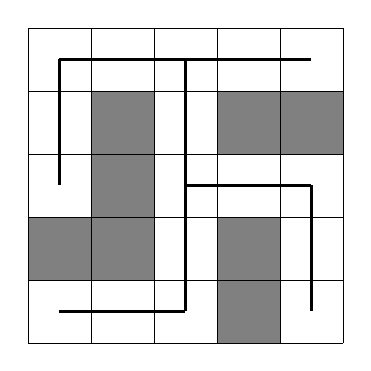
\begin{tikzpicture}[scale=0.8, every node/.style={circle,draw,minimum size=8mm}]
            \draw[very thick, black] (0.5,0.5) -- (2.5,0.5);
            \draw[very thick, black] (2.5,0.5) -- (2.5,4.5);
            \draw[very thick, black] (0.5,4.5) -- (4.5,4.5);
            \draw[very thick, black] (0.5,4.5) -- (0.5,2.5);
            \draw[very thick, black] (4.5,2.5) -- (4.5,0.5);
            \draw[very thick, black] (2.5,2.5) -- (4.5,2.5);

            \fill[gray] (0, 1) rectangle ++(1,1);
            \fill[gray] (1, 1) rectangle ++(1,1);
            \fill[gray] (1, 2) rectangle ++(1,1);
            \fill[gray] (1, 3) rectangle ++(1,1);
            \fill[gray] (3, 3) rectangle ++(1,1);
            \fill[gray] (4, 3) rectangle ++(1,1);
            \fill[gray] (3, 0) rectangle ++(1,1);
            \fill[gray] (3, 1) rectangle ++(1,1);

            \draw[step=1cm,ultra thin,black] (0,0) grid (5,5);
        \end{tikzpicture}
        \caption{\centering Wyznaczanie kolejnych krawędzi labiryntu.}
        \label{fig:prim_later_steps_a}
    \end{subfigure}
    \begin{subfigure}{0.45\textwidth}
        \centering
        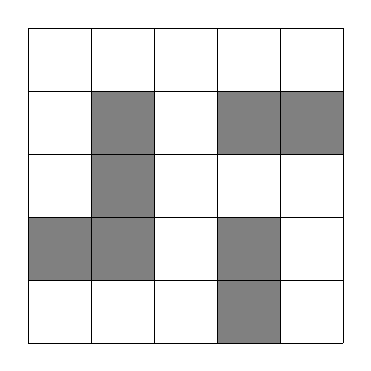
\begin{tikzpicture}[scale=0.8, every node/.style={circle,draw,minimum size=8mm}]
            \fill[gray] (0, 1) rectangle ++(1,1);
            \fill[gray] (1, 1) rectangle ++(1,1);
            \fill[gray] (1, 2) rectangle ++(1,1);
            \fill[gray] (1, 3) rectangle ++(1,1);
            \fill[gray] (3, 3) rectangle ++(1,1);
            \fill[gray] (4, 3) rectangle ++(1,1);
            \fill[gray] (3, 0) rectangle ++(1,1);
            \fill[gray] (3, 1) rectangle ++(1,1);

            \draw[step=1cm,ultra thin,black] (0,0) grid (5,5);
        \end{tikzpicture}
        \caption{\centering Labirynt powstały na podstawie wyznaczonych krawędzi.}
        \label{fig:prim_later_steps_b}
    \end{subfigure}
    \caption{Kolejne kroki działania algorytmu.}
    \label{fig:prim_later_steps}
\end{figure}